
% this file is called up by thesis.tex
% content in this file will be fed into the main document

%: ----------------------- introduction file header -----------------------
% the code below specifies where the figures are stored
\graphicspath{{3/figures/}}

\chapter{Deep Learning}
\label{chp:background}
% This article is structured very well: http://www.toptal.com/machine-learning/an-introduction-to-deep-learning-from-perceptrons-to-deep-networks
% Goals:
%  - Provide contextual background for deep networks (how did we get here)
%  - Equate traditional digital signal processing and deep learning
%  - Define the necessary pieces of deep learning

% Outline
%  - Background
%   -- Origins
%   -- Breakthroughs
%   -- State of the Art / recent developments
%  - Formal Definitions
%   -- What is ``deep learning''; non-linear function, parameterized, differentiable, optimized to a given objective criterion.
%   -- Architectures
%    --- Affine Layers
%    --- Convolutions (2d, 3d)
%    --- Nonlinearities
%    --- Pooling
%   -- Energy-based Learning
%    --- Scalar objective criteria (Loss Functionals)
%    --- Stochastic Minibatch Gradient Descent
%   -- Tricks
%    --- Regularization & Sparsity
%    --- Parameter Initialization
%    --- Dropout
%    --- Data Augmentation
%  - Relationship to Audio DSP


Deep learning descends from a long and contested history of artificial intelligence, information theory, and computer science.
The goals of the this chapter are two-fold:
Section \ref{background} first offers a concise summary of the history of deep learning in three parts, detailing the origins, critical advances, and current state of the art of neural networks.

Afterwards, a formal treatment of deep learning is addressed:
Section \ref{sec:arch} introduces the architectural components of deep networks;
Section \ref{sec:learning} formally addresses the actual ``learning'' process;
Section \ref{sec:tricks} covers a handful of pertinent tricks of the trade, enabling the practical realization of such models;
and finally, Section \ref{sec:dsp} draws the relationships between this lineage and conventional approaches to digital signal processing.


\section{A Brief History of Neural Networks}

Despite the recent wave of interest and excitement surrounding it, the core principles of deep learning were originally devised halfway through the 20th century, grounded in mathematics established even earlier.
As a direct descendant of neural networks ---computational models with an ambitious moniker burdened by a tumultuous past--- the very mention of deep learning often ellicts several warranted, if suspicious, questions: What's the difference? What's changed? Why do they suddenly work \emph{now}?
Thus, before diving into a formal review of the deep learning and its various components, it is worthwhile to contextualize the research trajectory that has led to today.


\subsection{Origins (pre-1980)}
\label{subsec:origins}

For Western Europe and those in its sphere of influence, the Age of Enlightenment marked a golden era of human knowledge, consisting of great advances in many diverse fields, such as mathematics, philosophy, and the physical sciences.
Long had humanity contemplated the notions of consciousness and reasoning, but here brilliant thinkers began to return to and explore these concepts with resolve.
From the efforts of scholars like Gottfried Leibnitz, Thomas Hobbes, and George Boole, formal logic blossomed into its own mathematical discipline.
In doing so, it became possible to symbolically express the act of reasoning, whereby rational thought could be described by a system of equations to be transformed or even solved.

It was this critical development ---the idea of logical computation--- that encouraged subsequent generations to speculate on the apparent feasibility of artificial intelligence.
And, coinciding with the advent of electricity in the 20th century, mathematicians, philosophers, and scientists of the modern era sought to create machines that could \emph{think}.
While the space of relevant contributions is too great to enumerate here, there were a handful of breakthroughs that would prove integral to the field of computer science.
In 1936, Alan Turing devised the concept of a ``universal machine'', which would lead to the proof that a system of binary states, e.g. true and false, could be used to perform \emph{any} mathmatical operation \cite{Turing1936}.
Only a year later, Claude Shannon demonstrated in his \emph{master's} thesis that Boolean logic could be implemented in electrical circuits via switches and relays, forming the basis of the modern computer \cite{Shannon1937}.
Shortly thereafter, in 1943, Pitts and McCulloch constructed the first artifical neuron, a simple computational model inspired by discoveries in neuroscience \cite{Pitts1943}.
By coarse analogy to a biology, an artifical neuron ``fires'' when a weighted combination of its inputs eclipse a given threshold:

\begin{align*}
  f(\mathbf{x}~|~\mathbf{w}) = h(\mathbf{w}^T~\cdot~\mathbf{x})\\
  h(y) = \left\{
    \begin{array}{ll}
      1 : y \ge 0\\
      0 : y < 0\\
    \end{array}
  \right.
\label{eq:perceptron}
\end{align*}

\noindent Importantly, as shown in Figure \ref{fig:neuron_logic}, it was demonstrated that such a model could be used to reproduce Boolean operations, such as AND or OR.
Given the clear application to the field of computational logic, artifical neurons only further encouraged the pursuit of artificially ``intelligent'' machines.

% Perceptron!
On its own, an artifical neuron is only a general processing structure, and the parameters it takes will specify the precise behavior of the model.
Arriving at these parameters, however, was nontrivial and required manual derivation.
Thus, in 1957, Frank Rosenblatt's invention of the \emph{Perceptron} algorithm signficantly altered how artificial neurons were conceived \cite{Rosenblatt1957}.
Building upon the work of Pitts and McCulloch, the algorithm, given in \ref{alg:perceptron_fit}, offered an automated method of ``learning'' the parameters necessary to achieve binary classification over a collection of data:

\begin{algorithm}[H]
\caption{Find the optimal parameters for a Perceptron over a collection of data.}
\label{array-sum}
\begin{algorithmic}[1]
\Procedure{FitPerceptron}{$\mathbf{x}, \mathbf{y}, \eta, n_{max}$}
    \State $\mathbf{w} \gets \mathcal{0}_{D + 1, 2}$
    \State $\mathbf{e} \gets \mathcal{1}_{N}$
    \State $n \gets 1$
    \While {$|\mathbf{e}| > 0$ \textbf{and} $n < n_{max}$}
        \State $\mathbf{z} \gets f(\mathbf{x} | \mathbf{w})$
        \State $\mathbf{e} \gets \mathbf{z} - \mathbf{y}$
        \State $\mathbf{w} \gets \mathbf{w} + \eta (\mathbf{e}^T \cdot \mathbf{x})^T$
        \State $n \gets n + 1$
    \EndWhile
    \State Return $\mathbf{w}$
\EndProcedure
\end{algorithmic}
\end{algorithm}

\noindent The perceptron algorithm requires four inputs:
a matrix of observations, $\mathbf{x}$, corresponding to $N$ samples with $D$ dimensions;
a vector of binary class assignments, $\mathbf{y}$, in the set $\{0, 1\}$;
an learning rate parameter, $\eta$;
and an iteration limit, $n_{max}$.
Initializing the algorithm, the weights, $\mathbf{w}$, are set to a matrix of zeros, shaped $(D + 1, 2)$, an error, $\mathbf{e}$, is set to a vector of ones, and the iteration counter, $n$, starts from 1.
Then, in an iterative manner, binary outputs, $\mathbf{z}$, are computed from the perceptron function, $f()$, given in Eq. \ref{eq:perceptron}, the error is computed as the difference between class predictions and targets, and the weights are updated with a scaled version of the incorrectly classified inputs.
Note that the error vector, $\mathbf{e}$ is only non-zero where the predicted values are wrong, and thus the algorithm naturally terminates when all datapoints are classified correctly.
Alternatively, execution is halted once a fixed number iterations is reached.
An example of a perceptron's stopping condition is given in Figure \ref{fig:linsep}.
Here, a perceptron has separated two classes of data, drawn from different Gaussian distributions.
As the algorithm proceeds, the total error decreases until a decision boundary is found that correctly classifies the observed data.

\begin{figure}
\begin{centering}
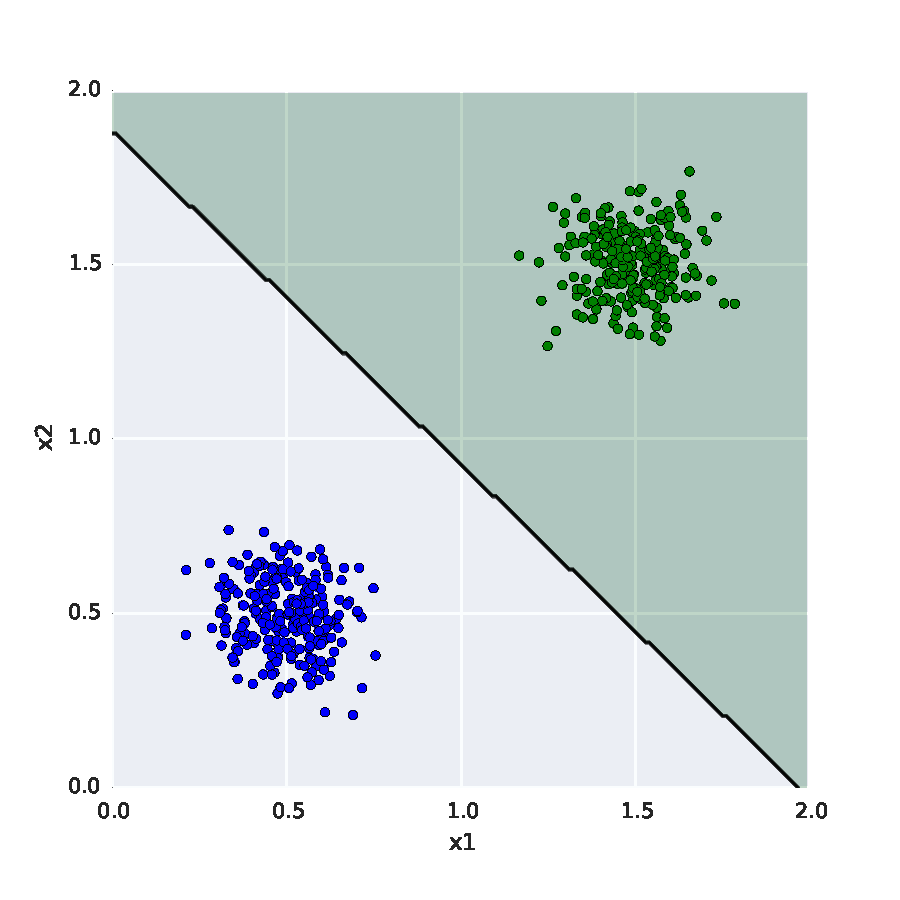
\includegraphics[width=0.6\textwidth]{linsep}
\caption{Linearly separable data classified by a trained perceptron.}
\label{fig:linsep}
\end{centering}
\end{figure}

% Promise and limitations
Once implemented in hardware, using a slew of potentiometers, motors, and photocells, Rosenblatt's' ``Mark I Perceptron'' drew considerable attention from the press and the research community alike.
The \emph{New York Times} was quick to publish ambitious claims as to the promise this breakthrough held for artificial intelligence and the speed at which subsequent advances would be realized, much to the eventual chagrin of the AI community \cite{somebody}.
However, the Perceptron was not without limitations nor critics.
In their book, \emph{Perceptrons}, published in 1969, Minsky and Papert demonstrated that the model is rather limited in the kinds of behavior it can actually achieve.
For example, perceptrons are unable to reproduce the logic of an exclusive-or (XOR), and thus can only classify \emph{linearly separable} data, the condition where a single straight line can be drawn between two classes.
% This scenario is illustrated in Figure \ref{fig:mlp_ftw}, where no single line can be draw to correctly classify the data.

% Multilayer Perceptrons
This was a critical limitation for researchers in the field of neural computation; if a perceptron could not perform basic logic operations, how could it be expected to reason?
The answer, as it would turn out, could be found by transforming how the XOR function is expressed symbolically.
Rearranging terms, an equivalent function can be rewritten as the disjuction (OR) of two complementary conjuctions (AND):

\begin{equation}
\label{eq:xor}
p \oplus q = (p \wedge \neg q) \vee (\neg p \wedge q)
\end{equation}

\noindent While it is true that a single Perceptron cannot achieve the XOR operation directly, a combination of \emph{three} can: two are used to perform each AND operation and corresponding negation, while a third performs the OR operation.
Considering the scenario in Figure \ref{fig:mlp_ftw}, this condition can now be easily separated by a \emph{multilayer} perceptron (MLP).
Therefore, arbitrarily complex functions could be obtained by cascading simpler non-linear operations, leading to a class of functions that would come to be known as \emph{neural networks}.
These models are so versatile, in fact, it would later be shown by the \emph{universal approximation theorem} that a neural network is actually able to model \emph{any} continous function, within some error tolerance \cite{Cybenko1989, Hornik1991}.

\begin{figure}
\begin{centering}
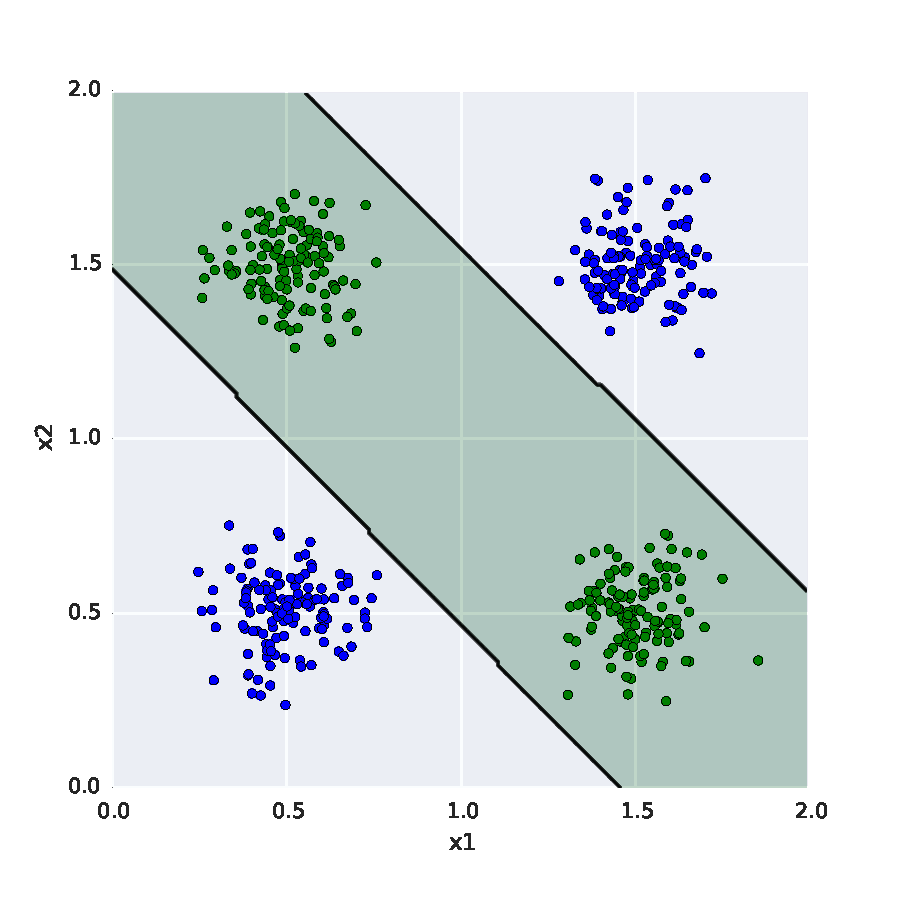
\includegraphics[width=0.6\textwidth]{mlp_ftw}
\caption{Demonstration of the decision boundaries for a \emph{multi-layer} perceptron.}
\label{fig:mlp_ftw}
\end{centering}
\end{figure}

% Other problems
Despite this promising observation, neural network research languished through the closing decades of the 20th century, suffering a considerable drop in funding support and, as a result, interest.
While the representational power of multilayer perceptrons was recognized early on, it became popular opinion that these models could not be used to solve complex problems.
In addition to theoretical skepticism, those who continued to pursue neural network research were also faced with an array of practical challenges.
Neural networks were prone to over-fitting, extremely slow to train, and difficult to use with more than a few layers.
% Ahead of the times
% Theory outpaced technological capacity. Over-hyped
Independently, these issues might merely have been viewed as common research obstacles.
However, coupled with the failed promises of early progress, such difficulties would malign the pursuit of neural network research for some time.
% This resulted in what is affectionately known as one of the ``AI winter'', things got bad.


\subsection{Scientific Milestones (1980--2010)}
\label{sec:advances}

In the face of widespread pessimism toward neural computing, some researchers would persevere through this ``AI Winter''.
Over the course of thirty some years, these diligent efforts would result in crucial breakthroughs that, in combination with the steady churn of technological progress, would fundamentally change the landscape of neural network research.
While no one facet can truly be credited with reviving the field, each would play an integral role in helping the research community again warm up to neural networks.

\subsubsection{Stochastic Gradient Descent}
\label{subsec:sgd}

% Back-propagation of errors
Via the perceptron algorithm, a machine effectively ``learns'' to classify data by finding parameters that optimize a given objective function.
This learning strategy must be modified in the multilayer case, as it is not possible to directly update the parameters through the heaviside, or unit step, function.
Early researchers noted that if the discontinuous activation function is replaced with a logistic, or sigmoid, the composite multilayer network is \emph{differentiable}.
Computing a model's fitness as a scalar \emph{loss}, this value can be differentiated with respect to every parameter in the function, thus \emph{back-propagating} error through the network \cite{Hinton1986}:

\begin{equation}
\label{eq:xor}
\frac{\partial~\mathcal{L}}{\partial~\Theta}  = ?
\end{equation}


% Issues of gradient descent
% This is a critical Once you can differentiate the network, gradient methods can be used to optimize the parameters.
Error back-propagation demonstrated that, so long as a network was everywhere differentiable, it was theoretically possible to optimize the objective function over a dataset by slowly adjusting parameters towards better solutions.
Framed as a minimization problem, a model's error can be incrementally decreased by taking small steps toward better parameters.
This optimization method, referred to as \emph{gradient descent}, was not without its deficiencies, however.
First and foremost, the loss of a given configuration was typically computed over the entire dataset, which may prove computationally expensive for sufficiently large collections.
Additionally, gradient descent is a greedy search algorithm, and was reportedly prone to finding poor local minima, as illustrated in Figure \ref{fig:local_min}.

\begin{figure}
\begin{centering}

\includegraphics[width=0.4\textwidth]{pink_muffin}
\caption{Gradient descent, yo.}
\label{fig:local_min}
\end{centering}
\end{figure}

%Stochastic Gradient Descent
In 1987, however, LeCun demonstrated that a \emph{stochastic} variant of gradient descent could potentially be used to circumvent these issues \cite{LeCun1987}.
Whereas conventional gradient descent had been formulated as an optimization over an entirely collection of datapoints, this new version randomly sampled training samples from a collection and computed an update step based on single datapoint.
Though the gradient is much noiser, this strategy is still effective,significantly faster, and may even be less susceptible to poor local minima as a result.
Importantly, this notion can be generalized as \emph{mini-batch} gradient descent, where the number of datapoints used to compute parameter updates is a hyperparameters, varying from 1 to the total number of datapoints available for training.
Covarying inversely with the learning rate, illustrated in Figure \ref{fig:sgd}, larger batch sizes serve to smooth parameter updates as a function of iteration.

\begin{figure}
\begin{centering}

\includegraphics[width=0.4\textwidth]{pink_muffin}
\caption{\emph{Stochastic} gradient descent, yo.}
\label{fig:local_min}
\end{centering}
\end{figure}

\subsubsection{Convolutional Neural Networks}
\label{subsec:convnets}

% Fully connected networks, bleh; sensitive to translation and scale
% TODO: Needs a better context sentence

Though equal parts remarkable and encouraging, the universal approximation theorem says nothing about how one might parameterize a neural network to achieve some desired behavior.
Thus, despite such overwhelming promise, early neural networks often resulted in poor approximations of the functions being modeled, because the flexibility of the model vastly surpassed the amount of data available to train it.
This flexibility was apparent in computer vision tasks, as multilayer perceptrons struggled to cope with simple homographic deformations, such as translation, scaling, or rotation.

% Visual cortex, neocognitron
Natural vision systems, on the other hand, are quite robust to these kinds of variation, and, as before, researchers looked to biology for inspiration in modeling these processes.
One particularly crucial study was that of Hubel and Wiesel in 1959, who experimented on the neural behavior of the feline visual cortex \cite{}.
By presenting visual stimuli while probing the brain with electrodes, they discovered two different kinds of neurons ---simple cells and complex cells--- organized hierarchically.
Experimental results indicated that the former is responsible for local feature extraction, while the latter combines the inputs of simple cells to absorb small amounts of variation in the observed stimuli.

% ConvNets, LeNet5, handwritten digits
These ideas were first incorporated in the Neocognitron of \cite{Fukushima1988}, and realized successfully as a convolutional neural network for shape recognition and handwritten digit classification \cite{LeCun1990, LeCun1998},  offering three key design features.
\emph{Local receptive fields}, where compute features from a small neighborhood of pixels, exploiting the observation that nearby pixel values tend to be highly correlated.
Smaller receptive fields require fewer parameters, thus reducing the overall size of the model and the amount of data needed to train it.
Applying local receptive fields as a convolution results in effectively sharing the weights over all positions in an image.
Thus \emph{weight sharing} reduces the number of parameters even further, while allowing the network to identify features regardless of position in an image.
Finally, \emph{max-pooling} reduces small neighborhoods to the largest value within it, introducing not only shift but a small amount of scale and rotation invariance.
Taken together, these advantageous attributes directly resolved many of the issues plaguing multilayer perceptrons, and proved to be the most successful instance of neural computing for nearly two decades.


% Theory preceded data
\subsubsection{Proliferation of Digital Data}
\label{subsec:perceptrons}

% Early data
Given the ubiquity of digital information in the modern era, it is easy to forget that neural networks were first developed in a considerably different day and age.
The very existence of digital audio and images, for example, did not become commonplace until the end of the 20th century.
Even then, these signals were costly to create, cumbersome to work with, and generally difficult to share.
Furthermore, once obtained, the process of annotating this information for use in supervised learning requires a great deal of time and effort.
Thus, in the vein of speech recognition or computer vision for example, machine perception research was forced to work with small datasets as a result.
Given the versatility of neural networks to model complex data, it was typically trivial to \emph{over-fit}, e.g. master, a small number of training examples, while failing to generalize to new data.
Neural networks developed the reputation of being ``data hungry'', requiring a large amount of training data in order to do anything useful in practice.

% Labeled datasets grew, intentionally or otherwise
While this was, and in some cases still is, a valid consideration for neural networks, the problem of data scarcity is far less of an issue now.
For many well worn tasks, researchers have had ample time to curate massive labeled datasets.
In the late 1980s, LeCun et al oversaw the development of a handwritten digit dataset, comprised of 60k 28x28 pixel images \cite{};
for comparison, the ImageNet dataset consists of millions of tagged, high resolution images \cite{}.
Similar efforts have been undertaken in the fields of speech recognition \cite{TIMIT}, source separation \cite{charm, MedleyDB}, or natural language processing \cite{WallStreet, Wikipedia}, to name only a few.
Additionally, given the rise of the Internet, it became possible to leverage a variety of information sources to obtain labeled data, such as user-generated content \cite{last.fm}, weak feedback signals \cite{netflix}, or even as a means of distributing the annotation effort \cite{Captcha, CitizenScience}.
Combined, the range of information available for large-scale supervised learning grew considerably, diminishing the issues posed by data-hungry algorithms.

% unlabeled data has uses too
However, as a by-product of the global transition to the digital realm, an even larger portion of \emph{unlabeled} data was at the disposal of machine learning researchers.
Coupling the easy availability of digital information with the idea that ``the human brain isn't \emph{really} supervised'', much effort was invested in the space of \emph{unsupervised} learning algorithms. %, i.e. learning from unlabeled data.
Finally, in 2006, one such method, referred as \emph{contrastive divergence}, was able to successfully exploit unlabeled data to improve the performance of a neural network.
Using a cascade of of undirected models, known as a Restricted Boltzmann machine (RBM), a neural network was trained in a greedy, layer-wise manner to reproduce realistic data.
After this process of learning how real data behaves, the model could be ``fine-tuned'' with a small amount of labeled data to realize impressive, state of the art performance.
Referred to as ``pre-training'', learning on unsupervised data allowed the model to discover parameters closer to a good final solution.
Though later discoveries would demonstrate pre-training to be unnecessary under certain conditions \cite{}, this breakthrough was perhaps the first to forcefully recapture the attention of the machine learning community.

% Subsequently, similar unsupervised approaches
%  called an autoencoder \cite{Vincent2010}, or ---an alternative interpretation from another research team--- Predictive Sparse Decomposition \cite{Ranzato2007}, incorporates roughly the same principles with deterministic interpretation of these concepts.
% In either view of the parameter optimization problem, learning algorithms now exist that can leverage large quantities of unlabeled data to tune large networks with minimal supervision.
% These advances have collectively ushered in a new era of machine learning, referred to as \emph{deep learning}, named so for the multiple levels of information processing and the manner in which the parameters of the system are discovered from data.


% Theory preceded technology
\subsubsection{Advances in Computing Technology}
\label{subsubsec:hardware}

% Neural networks were devised in the 60s; in the 80s, computers sucked
While enough cannot be said about the scientific contributions of neural network researchers over the last 40 years, it is critical to appreciate how computing technology has evolved over that time span.
In the days of Rosenblatt and Minsky, computers consisted of transistors that were visible to the naked eye, filled entire rooms, and cost a small fortune.
More recently, personal computers of the 1980s had kilobytes of memory, central processing units (CPUs) operated in the range of tens of megahertz, and were still far too expensive for all but the elite or dedicate.
Computation was still quite slow as a result, and thus the process of traning neural networks took an impressive amount of time.
To combat these difficulties, researchers often attempted to cut corners by using smaller models, smaller datasets, and training with fewer iterations.
Somewhat unsurprisingly, the common experience with neural networks was quite unfavorable.

% Now better; bigger hard disks, more memory, faster processors, GPUs, async SGD, distributed computing, better tools (Theano, Torch)
Eventually, though, technology could catch up to the theory.
Hardware became increasingly smaller, memory grew to the size of gigabytes, processors accelerated for a time without bound faster, and the cost of computers dropped to the point of near ubiquity.
On the heels of these developments, other hardware and tools were adapted to facilitate neural network research, such as parallel computing with graphics processing units (GPUs) and accessible software tools, e.g. Theano\footnote{} or Torch\footnote{}.
Combined, singificantly better technology directly enabled research at unprecedented scale, accelerating progress and relaxing computational constraints imposed by technical limitations.

% Additionally, significant increases in computational power, and especially advances in parallel computing via GPUs, make deep learning not only feasible, but in some cases an efficient approach to research.
% Evidenced by the recent work of \cite{kittehs}, some are beginning to attempt large scale deep learning on unprecedented quantities of data.
% Similarly, software libraries and toolkits \cite{Theano, Torch, Caafe} are now available that leverage these computational gains to make deep learning more accessible to the entire research community.


\subsection{Modern Rennaissance (post-2010)}
\label{subsec:rennaissance}

% Industrial strength; Google, Facebook, Baidu, Microsoft
Following the many key advances named above, deep learning quickly accelerated into the academic, industrial, and public lexicon.
It did not take long to convince some research communities of the newfound promise of neural networks.
In hardly any time at all, deep neural networks surpassed the state of the art in automatic speech recognition, systems tuned over the course of several decades \cite{Hinton2009}.
Similarly compelling results were obtained in computer vision, such as recognizing house numbers from Google Street View images \cite{} or the image labeling challenge known as ImageNet \cite{}, and natural languange processing \cite{Sutskever2010}.
Acknowledging the usefulness of such high-performing systems, companies like Google, Facebook, Microsoft, IBM, and Baidu began investing in industrial strength deep learning teams and infrastructure \cite{Dean2012, LeCun2014}.

Complementing the migration of ideas and individuals from academia to industry, the idea of ``deep learning'' and thinking machines has again struck a chord with both the press and general public.
Google's research efforts in 2012, for example, yielded a deep network that automatically learned the concepts of ``cats'' and ``human faces'', trained on millions of still video frames from YouTube \cite{Le2012}.
Understandably, the story was picked up by \emph{The New York Times} and \emph{WIRED}, among countless others, drawing widespread attention.
Coupled with charistmatic interviews from many of the field's preeminent leaders, neural networks have been thrust back into the limelight. %again captured the minds and imaginations of many.


\section{Core Concepts}
\label{sec:example}

% The "what" of deep learning
% One takeaway that should result from this historical review,
Reflecting on the historical lineage of neural networks, it becomes apparent that deep learning is not one single thing, but rather a collection of ideas and approaches toward neural computing.
Thus, to help define the scope and limits of this work, this section introduces the fundamental components that contribute to a modern definition of the topic.
Here, ``deep learning'' is defined as an approach to designing complex information processing systems, exhibiting two key traits;
one, discussed in Subsection \ref{subsec:architectures}, the system architecture can be expressed as a composite nonlinear function, composed of many simpler operations;
and two, presented in Subsection \ref{subsec:learning}, the parameters of this function can be ``learned'' by combining an objective function with numerical optimzation methods.
Finally, modern neural network research has produced a useful array of ``tricks of the trade'', detailed in Subection \ref{subsec:tricks}, which often help squeeze every bit of performance from a model.


\subsection{Modular Architectures}
\label{subsec:architectures}

% Building blocks of neural networks.
It is a hallmark of deep neural networks that system architectures are constructed from only a handful of unique processing units, repeated and arranged to form complex structures.
This modular approach to system design allows the researcher to focus on each operation at different levels of abstraction;
from a few basic building blocks, it is straightforward to create elaborate architectures \cite{inceptionnet}.
While any mathematical operation can be easily incorporated into a neural network, so long as it is differentiable, there are a handful of common operations that are worth discussing.

\subsubsection{Composite Architectures}

Conventionally, a neural network transforms an input $X_{1}$ into an output $Z_{L}$ via a composite nonlinear function $F(\cdot \vert \Theta)$, given a parameter set $\Theta$.
This is traditionally, but not necessarily, achieved as a cascade of $L$ self-contained operations, $f_l(\cdot \vert \theta_l)$, referred to as layers, nodes, or subfunctions, the order of which is indexed by $l$:

\begin{equation}
\label{eq:layers}
F(X_{1} \vert \Theta) = f_{L}(  ... f_2(f_1(X_{1} \vert \theta_1) \vert \theta_2) ) ... \vert \theta_{L})
\end{equation}

\noindent In this formulation, $F = [f_1, f_2, ... f_{L} ]$ is the set of layers, $\Theta = [\theta_1, \theta_2, ... \theta_{L} ]$ is the corresponding set of parameters, the output of one layer is passed as the input to the next, as $X_{l+1} = Z_{l}$, and the overall \emph{depth} of the network is given by $L$.

It is worth noting that this sequential cascade of operations is merely common practice and not a hard and fast rule.
Some networks make use of interesting types of connectivity between layers, referred to as ``skip-connections'' \cite{LeCun};
others adopt an explicit graphical interpretation, encouraging the description of the network in terms of nodes and edges.
Therefore the design of a network architecture must address several interrelated questions:
what is the function being modeled?
what domain knowledge can be leveraged to inform this design?
and how do these relate to the data being processed, or the problem being addressed?
The considerable flexibility afforded by this modular design approach is both one of the greatest advantages, and criticisms, of deep neural networks.


\subsubsection{Affine Projection}

The fundamental building block of the classic neural network is the affine transformation:

\begin{equation}
\label{eq:fclayer}
Z_l = f_l(X_l \vert \theta_l) = h( W \bullet X_{l} + b), \theta_l = [W, b]
\end{equation}

\noindent Here, the input to the $l^{th}$ layer, $X_l$, is flatten to a column vector of length $N$, projected against a weight matrix, $W$, of shape $(M, N)$, added to a vector bias term, $b$, of length $M$, and passed through some transfer function, $h()$.
As addressed shortly, the transfer function is generally some pointwise nonlinearity, although the linear matrix product can be seen as a special case of Eq. \ref{eq:fclayer}.
Alternatively, this operation is also known as a fully-connected or matrix-product layer.
This common subfunction descends directly from the perceptron, and is the core operation of the multi-layer perceptron.
Additionally, the affine transformation is a crucial processing block, because, as it will soon be discussed, many other subfunctions can be interpreted as a special instance of a matrix-product.


\subsubsection{Local Affine Transformation}

% Local Receptive Fields
% Fully connected matrices that are only connected to local neighborhoods.
Though somewhat out of order chronologically, the nearest neighbor to an affine transformation in the realm of deep learning is the ``local affine transformation'' \cite{someone}, operating only on local neighborhoods.
Based on observations of visual systems, local receptive fields exploit correlations found in spatial pixel neighborhoods to reduce the complexity of features to be learned, generally resulting in better performance \cite{who}.
Notably, local affine transformations can be realized as a full matrix product where most weights are zero, expressed as the following:

\begingroup
\renewcommand*{\arraystretch}{0.8}
$$
\begin{bmatrix}
w_{0, 0} & w_{0, 1} & \dots  & w_{0, M} & 0 & \dots & 0 & 0 \\
w_{1, 0} & w_{1, 1} & \dots  & w_{1, M} & 0 & \dots & 0 & 0 \\
\vdots & \vdots & \ddots & \vdots & 0 & \ddots & 0 & 0 \\
w_{K, 0} & w_{K, 1} & \dots  & w_{K, M} & 0 & \dots & 0 & 0 \\
0 & w_{K + 1, 1} & w_{K + 1, 2} & \dots  & w_{K + 1, M + 1} & 0 & \dots & 0 \\
\vdots & \vdots & \vdots & \ddots & \vdots & 0 & \ddots & \vdots \\
0 & w_{2K, 1} & w_{2K, 2} & \dots  & w_{2K, M + 1} & 0 & \dots & 0 \\
0 & \ddots & \vdots & \vdots & \ddots & \dots & \dots & 0 \\
\dots & 0 & w_{i, j} & w_{i, j + 1} & \dots & w_{i, j + M} & 0 & \dots \\
\dots & 0 & w_{i + 1, j} & w_{i + 1, j + 1} & \dots & w_{i + 1, j + M} & 0  & \dots  \\
\dots & 0 & \vdots & \vdots & \ddots & \vdots & 0 & \dots \\
\dots & 0 & w_{i + K, j} & w_{i+K, j + 1} & \dots & w_{i + K, j + M} & 0  & \dots  \\
\dots & \dots & \dots & \dots & \dots & \dots & \dots & \ddots
\end{bmatrix}
$$
\endgroup

\noindent Here, $M$ adjacent features are projected against $K$ different combinations of weights, and this local connectivity is translated across all possible locations of a given input.
This formulation is particularly interesting, as it illustrates the inherent difficulty posed by the universal approximation theorem.
Technically, a local receptive field can be implemented as a matrix-product;
learning this behavior, however, is quite difficult.
First off, this particular sparse connectivity would need to be learned redundantly.
Additionally, such true sparsity is challenging to learn, and it is unlikely such behavior would be so well localized.
Finally, the prospect of learning this particular topology from a fully-connected matrix demands a prohibitive number of parameters, throttling both computation and the learning process.

Furthermore, this spatially correlated topology is unique to visual signals, and such connectivity assumptions may not map to other domains.
Natural sound, for example, is harmonic in nature, and it is reasonable to assume that octave relationships may have a stronger connection that neighboring frequencies.
Some research has argued that different types of connectivity could be determined from data \cite{Coates2012?}, but this has yet to be extensively explored in the deep learning literature.


\subsubsection{Convolutions}

Extending the topology of local receptive fields, convolutions further simplify this process by sharing the \emph{exact} same parameters across location in an input representation.
Also known as weight tying, a convolution is generically expressed by the following:

\begin{equation}
\label{eq:convlayer}
\small
f_l(X_l \vert \theta_l) = h(X_{l} \circledast W + b), \theta_l = [W, b]
\end{equation}

\noindent In deep learning literature, there are typically two kinds of convolution operations indicated by the $\circledast$.
The first, and perhaps original, interpretation is referred to as a ``2D'' convolution:

\begin{equation}
\label{eq:convolution}
\small
\hat{Z}[m, a, b]_l =\sum_{i=0}^{N} \sum_{j=-\infty}^{\infty} \sum_{k=-\infty}^{\infty} X_l[i, x, y]W[m, a - j, b - k]
\end{equation}

\noindent Here the convolution is computed by convolving a 3D input tensor, $X$, consisting of $N$ \emph{feature maps}, with a collection of $M$ 2D weight \emph{kernels}, $W$, followed by the addition of a vector bias term $b$.
In this formulation, $X$ has shape $(N, d_0, d_1)$ where $(d_0,d_1)$ is the shape of each map, $W$ has shape $(M, m_0, m_1)$, where $(m_0,m_1)$ define the size of the kernel.
Note that in the 2D formulation, the activation of a kernel is summed equally across the separate feature maps, and thus the degrees of freedom for such a kernel are across spatial and feature map dimensions.

Alternatively, the other common variant of the $\circledast$ operator is the 3D convolution, written as follows:

\begin{equation}
\label{eq:convolution}
\small
\hat{Z}_l[m, a, b] =\sum_{i=0}^{N} \sum_{j=-\infty}^{\infty} \sum_{k=-\infty}^{\infty} X[i, x, y]W[m, i, a - j, b - k]
\end{equation}

\noindent The input, $X$, is again a 3D tensor of feature maps, but now the weight tensor used in the convolution, $W$, is 4D, with shape $(M, N, m_0, m_1)$.
Whereas before, in the 2D case, each kernel translated across feature maps, the 3D case aligns a kernel with the number of feature maps, $N$.
Thus, in the instance that $N=1$, both operations are equivalent.
Due to the local connectivity across feature maps, 3D convolutions require $N$ times more parameters than their 2D cousin, but far fewer than an equivalent full matrix product.
Using kernels that are sensitive to characteristics across different simultaneous feature maps allows for correlations to be discovered across the same representation.


% There are two primary benefits to using convolutional layers in a deep network; the number of parameters to learn is greatly reduced because only a local neighborhood, rather than the entire input, is processed by each kernel; and two, the kernel is translated across all shifts of the input, allowing it to encode the same feature regardless of absolute position; we refer the interested reader to \cite{LeCun2010} for a more extensive review.


% \subsubsection{Recursive Operations}
% Is this even necessary?
% Related to HMMs, stateful
% Notoriously difficult to train
% Unroll a fixed number of steps, with burn in
% Echo state networks
% Heuristics: LSTM, gradient clipping
% Various mileage.


\subsubsection{Nonlinearities}

A seemingly simple piece of the deep learning toolkit, pointwise nonlinearities are crucial to the construction of complex networks.
In the absence of nonlinear behavior, a cascade of linear systems is itself another linear system.
Nonlinear operations, however, change the overall behavior of the composite function, and are the source of representational power in deep networks.
Conventionally referred to as \emph{transfer} or \emph{activation} functions, these operations are typically applied to the output of other linear functions, e.g. after an affine transformation.

The two basic nonlinear functions in deep networks are the logistic, or sigmoid, and the related hyperbolic tangent:

\begin{align*}
  logistic(x) = \frac{1}{1 + \mathrm{e}^{-x}}\\
  tanh(x) = \frac{1 - \mathrm{e}^{-2x}} {1 + \mathrm{e}^{-2x}}
\label{eq:basic_nonlinearities}
\end{align*}

Shown in Figure \ref{fig:nonlinearities}, both functions have inflection points at zero, saturate toward infinity in both directions, and are everywhere differentiable.
While the logistic initially came into practice as a smooth approximation to the unit step function, the hyperbolic tangent has gained favor for being centered about the origin.
The saturating behavior of these functions is significant, because training a poorly initialized network may be painfully slow, if even possible, due to small gradients at the limits.

More recently, the \emph{Rectified Linear Unit} (ReLU), or halfwave rectification, has seen a considerable uptick in usage in deep networks:

\begin{align*}
  relu(x) = max(x, 0) = x * (x > 0)\\
\label{eq:relu}
\end{align*}

% piecewise linear model. % relationship to random forests?
\noindent Notably, it was demonstrated in \cite{Hinton} that, with sufficient data, rectified linear units could achieve state of the art performance without unsupervised pretraining.
Though the theory is still catching up to the practice, there are two widely held rationalizations of this behavior.
Most importantly, the function does not saturate in the positve region, and thus gradients propagate freely through an arbitrarily deep network.
Additionaly, the hard threshold results in naturally sparse representations, a ``good thing'' in classification systems.
Noting that no information flows in the negative mode, others have extended this idea into the ``leaky ReLU'', but these have not see such widespread attention \cite{Ng?}.

% Full wave rectification, soft approximations?
% Shrinkage functions, common in sparse coding
% Any differentiable nonlinearity could conceivably be used here.


\subsubsection{Pooling}

% Pooling

In a broad sense, \emph{pooling} operations compute local statistics over representations.
This can be understood as a form of summarization, which trades accuracy of locality for various forms of invariance.
Original drawing inspiration from the Hubel and Weisel experiments, the most common pooling operation is \emph{max-pooling}, which mimics the behavior of complex cells in the visual cortex by passing only the largest value within a local neighborhood.
This offers, depending on the size of the neighborhood, invariance to scale, translation, and rotation in visual tasks, and contributes significantly to the success of convolutional networks.
the parameter $p_0, p_1$ is a two-element tuple that defines the neighborhood of the max operator along these dimensions:


\begin{equation}
\label{eq:maxpool}
\small
\hat{Z}[x, y] = max (\mathcal{1}_{p=0}^{P} \mathcal{1}_{q=}^{Q} X[x + p, y + q]
\end{equation}

% \noindent This would later find use in \emph{max-out networks}, where the adjacent outputs of an affine transformations are max-pooled \cite{Goodfellow2011}.
% The difference here being that conventional pooling exploits spatial correlations

Other forms of pooling exist, though less common in practice.
Similar in nature, \emph{L2-pooling} computes the magnitude vector of a neighborhood in Euclidean space \cite{LeCunStudent}.
This can be interpreted as a softer form of max-pooling, where all inputs contribute to the output, albeit dominated by the maxima.
Finally, other statistics like the \emph{mean}, \emph{min}, or \emph{standard deviation} have found use in temporal pooling \cite{Hamel2011}.


\subsubsection{Constraints}

Given the many degrees of freedom that can be realized with neural networks, it is often necessary to constrain representations to behave in certain ways.
%Softmax
Perhaps the most common instance of this is found in classification systems, where the output of a network estimates the likelihood or affinity for some number of classes.
The \emph{maximum a posteriori}, or MAP, decision rule is a particularly simple, and thus attractive, one in this case, which identifies the maximum likelihood as the winning class.
Traditionally, the probability mass function $P(\cdot)$ for an input $X_1$ is achieved by applying the softmax operation to the output of the network, $Z_L$, defined as follows:

\begin{equation}
\label{eq:softmax}
\sigma(X) = \frac{\exp(\beta X)}{ \sum_{k=1}^{K}\exp{(\beta X_k)}}
\end{equation}

\noindent Again, note that $X$ is the output of the final layer, $f_L$, and thus $K$ is the dimensionality of the classifier and equal to the number of classes in the problem.
Therefore, the most likely class for a prediction $Z$, is given by $k = argmax(\sigma(Z))$.

% L2 constraints, bounded in volume, bounded to surface.


\subsection{Automatic Learning}
\label{subsec:learning}

Having defined a deep network, it is necessary to determine an approach to finding parameters that enable this general function to perform some specific behavior.
The deep learning is two-fold: define an objective function, and optimze to it over a collection of training data.


\subsubsection{Objective Functions}

Energy based learning
Low-energy corresponds to likely states.
Define a loss functional (function that takes a function)
Enables inference

Here, a few loss functions of note are discussed; for a comprehensive review, the curious reader is directed to \cite{LeCun2006}.
% Perceptron Loss, error function
Basic error function is the perceptron loss:

\begin{equation}
\label{eq:nll}
\mathcal{L}_perceptron(Y_k | X, \Theta) = || Y_k - f(X | \Theta) ||_2
\end{equation}

\noindent Some comment about this thing.

% Negative Log-likelihood
Having written the full network as a probability mass function, the network can be trained by iteratively minimizing the negative log-likelihood of the correct class for a set of $K$ observations:

\begin{equation}
\label{eq:nll}
\mathcal{L}=-\sum_{k=0}^K log(P(X^k = Y^k \vert \Theta))
\end{equation}

\noindent Expressed in this manner, $X^k$ and $Y^k$ are the input data and corresponding class label, respectively of the $k^{th}$ observation.


\subsubsection{Numerical Optimization}

% Automatic methods
Learning should be automatic
Random, brute force, genetic algorithms fit the bill.
No reasonable expectation of finding a good answer.

% Gradient methods, a fighting chance
Gradient methods, while greedy, at least attempt to go toward better answers.
The basic idea being that a function attempts to reduce how ``wrong'' it is by taking small steps toward better answers; by analogy, this is a bit like climbing down a mountain blind-folded.
Specifically, the update rule for $\Theta$ is defined as its difference with the gradient of the scalar loss $\mathcal{L}$ with respect to the parameters $\Theta$, weighted by the learning rate $\eta$, given by the following:

\begin{equation}
\label{eq:updaterule}
\Theta \leftarrow \Theta - \eta * \frac{ \delta \mathcal{L}}{\delta \Theta}
\end{equation}

As shown in Figure \ref{fig:loss_surface}, this algorithm can be susceptible to bad local optima in highly non-convex surfaces.
There are additionally degenerate cases such that a first-order method like this may be very slow, and thus higher order methods BGFS, L-BGFS, have been devised to deal with such issues.
Higher order methods often entail a higher computational cost.
In practice however, gradient descent is often sufficent with some slight modifcations, such as the occasional computation of the Hessian \cite{} or Nesterov momentum.



\subsection{Tricks of the Trade}
\label{subsec:tricks}

%   -- Tricks
\subsubsection{Regularization \& Sparsity}
Reduce over-fitting via weight decay.
L2 penalties make values small without going to zero

Sparse representation are good.
L0 and L1 loss are closely related, will drive values all the way to zero.

\subsubsection{Data-Driven Initialization}

Core idea behind the first significant breakthrough of the modern era.
Get parameters of the network closer to a good solution.
Resolves poorly conditioned networks.
Alleviates the vanishing gradient problem.
Less important now, given relu's; still useful for problems which lack sufficient labeled data.


\subsubsection{Dropout}
Prevents co-adaptation of parameters \cite{Hinton2012}.
Related to model averaging.
Trains a subset of all networks at every iteration.
Reduces the theoretical bound on generalization error.


\subsubsection{Data Augmentation}

Get more mileage out of labeled data by applying known deformations.
Exploit the reality that modeling the synthesis process is typically easier than the analysis process.
LeCun 1998
Dieleman 2014 Kaggle, Galaxy Zoo


\subsubsection{Normalization}

%Enough can't be said about normalization

% Unit scaling

% Standardization

% Local contrast normalization


\section{Related Efforts in Automatic Music Description}

% NMF all the rage
Source separation

While far from widespread, an increasing number of researchers are investing more time and effort into the application of deep learning to challenges in content-based music informatics.
Deep Belief Networks quickly gained popularity for genre recognition \cite{Hamel2009}, mood estimation \cite{Schmidt2011}, note transcription \cite{Nam2011}, and artist recognition \cite{Dieleman2011}.

% Convolutional networks
Many early applications operate on single frame observations of a music signal.
Among the first uses of deep learning were the application of convolutional networks to the detection of onsets \cite{Lacoste2007}
Incorporating longer time-scales, convolutional networks have also been explored for, again, genre recognition \cite{Li2010}, instrument similarity \cite{Humphrey2010}, chord estimation \cite{Humphrey2011, Humphrey2012b}, and onset detection \cite{Schluter2014}.
Recursive networks have been explored for sequence modelling \cite{Boulanger2013} and pitch analysis \cite{Sigtia2014}.
\cite{Cherla2014}.
\cite{Durand2015}

% Recursive models
and long short-term memory to model symbolic music sequences \cite{Eck2008}.

% Other related stuff
Conditional networks were explored for rhythm pattern analysis \cite{Battenberg2012}.
Predictive Sparse Decomposition (PSD) and methods inspired by sparse coding have also seen a spike in activity over the last two years for a variety of tasks \cite{Henaff2011, Nam2012}, but despite being developed for deep learning, neither of these systems are actually hierarchical.

% Needs more from Sander, Aron van der Oord, Srikanth Cherla, Siddarth, Boulanger-Lewandowski

It is worthwhile to note that many, if not all, of these works have achieved state of the art performance on their respective tasks, often in the first application of the method to the area.
Any instances where this has occurred, however, deep learning techniques have simply been directly some kind of derived audio representation with minimal modification.
It is therefore important to realize that these methods have never been tailored to address the nuances of music signals, and more importantly time.
Overall, only CNNs make an effort to consider observations on the order of seconds, but do so in an admittedly awkward way, requiring the observation length be defined \emph{a priori}.
The machine is ultimately limited to the amount of information it sees in its analysis, and there is obviously no fixed duration in which all musical behavior resides.

% Due to advances in machine computation, there are primarily two different ways to conceptualize the design of information processing models.
% One approach is based on signal theory as viewed through the lens of electrical engineering, whereas the other focuses on graphical models of artificial neural processing grounded in computer science.
% Though broad topics of study in themselves, they are worth mentioning together for two crucial reasons: first, a majority of inertia developed within the field of MIR is due largely to its roots in the former; and second, it is a useful juxtaposition to form when marrying these disconnected topics.

%Electrical engineering formalized as a discipline in the middle of the $19^{th}$ century on the heels of inventions such as the telegraph and electric power distribution.

% Much early work in electrical engineering stemmed from the realization that electricity could be used to represent measurable phenomena and therefore capture, store, and transmit this information.
% These representations are referred to as analog signals because they use one representation ---time-varying voltage, for example--- to mirror another one ---such as a sound pressure wave--- in a continuous fashion.
% It was soon discovered that not only could this information be represented via electricity, but that it was also possible to analyze and manipulate it for a variety of applications.
% Heavily grounded in classic numerical analysis methods of the $17^{th}$ and $18^{th}$ centuries, these methods are referred to as signal processing.
% Through experimentation in physics, scientists found that certain electromagnetic materials could be used to affect electricity in predictable ways, and when connected in an electrical circuit could be used to filter, or augment, signals.
% Importantly, the need to solve signal processing systems by inspection requires that the entire system be linear and time invariant (LTI), because the violation of either property makes mathematical analysis far too difficult, if not altogether impossible.

% With the advent of solid-state transistors and subsequently computers in the mid-$20^{th}$, digital representations of signals could be produced by sampling analog waveforms to be manipulated numerically, referred to as digital signal processing (DSP).
% Digital signals---those that also represent some kind of real world phenomena, at least---differ from analog ones in two important aspects: the signal takes values from a finite set of discrete numbers, and these quantities are measured at precise moments in time.
% Therefore, digital signals are specified by a sequence of real-valued numbers $x[n]$, rather than a generated, continuous function $x(t)$.
% When this transition to numerical computation began, the effort was made to reformulate previous knowledge regarding analog signal theory and processing into the digital domain.
% Similar to those in analog theory, digital filters can be expressed explicitly by a transfer function, which can be translated directly to a set of coefficients representing the linear difference equation, generically given by the following:

% \begin{equation}
% \label{eq:diffeq}
% \begin{array}{rcr}
% y[n] & = & b_0x[n] + b_1x[n-1] + b_2x[n-2] + b_3x[n-3] \ldots \\
%  & & - a_1y[n-1] - a_2y[n-2] - a_3y[n-3] \ldots
% \end{array}
% \end{equation}

% There are typically said to be two categories of digital filters: Finite Impulse Response (FIR), or non-recursive, filters and Infinite Impulse Response (IIR), or recursive, filters.
% As illustrated in Figure \ref{fig:filters}, an FIR filter is actually a special case of the more general IIR filter, where the feedback connections---the $a$-coefficients in Equation (\ref{eq:diffeq})---have all been set to zero.
% Though digital filters are not constrained by the availability or precision of manufactured electrical components, they are still traditionally constrained to be LTI systems for the same reasons as their analog counterparts.
% As a result, non-linear signal processing models in both the analog and digital domains are historically unpopular due to inherent challenges in the mathematical formulation.

% \begin{figure}[!t]
% \centering
% 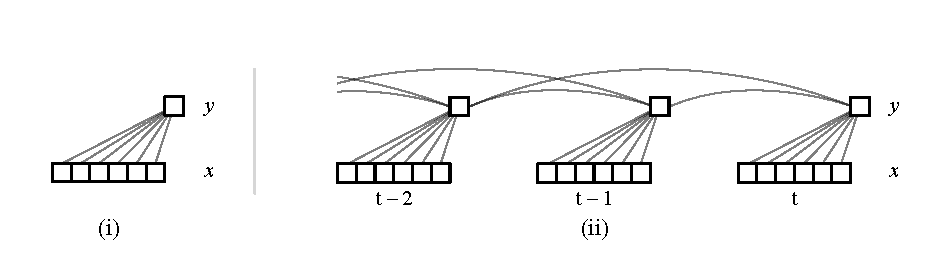
\includegraphics[width=\textwidth]{filters_2}
% \caption{\small{Finite Impulse Response (i) and Infinite Impulse Response (ii) digital filters. Multiplication is shown along the edges of each connection.}}
% \label{fig:filters}
% \end{figure}


% Looking closely at recent work in deep learning, most of the effort has been invested in areas of static input representations, i.e. computer vision and still images.
% As evidenced by music, audio, and video, time plays an extremely important role in the way that information is conveyed.
% Though CNNs have been applied to signals with a temporal dimension \cite{LeCun1994}, recursive architectures have shown promise for addressing the problem of time and sequences in data.
% Initial efforts to train RNNs however, even with supervised methods, proved extremely challenging, with the observed phenomena manifesting as numerical stability issues of the gradient.
% Due to the recursive nature of the model, backpropagating the error signal through time is prone to make the amplitude of the gradient either vanish or explode.
% Despite these difficulties, several approaches and optimization methods have been developed in recent years that encourage further exploration of these models.

% One of the earliest successful attempts to circumvent the issue of gradient stability was realized through a method called LSTM \cite{Schmidhuber1997}, where the gradient signal is ``latched'' by a hidden unit such that its information could be saved long enough to be useful.
% Similar notions surround the notion of reservoir computing, such as echo-state networks, which employ feedback connections to cache arbitrary temporal information such that a second non-recursive layer ---being far easier to train--- might be able to make sense of it \cite{Jaeger2002}.
% Alternatively, conditional DBNs have been employed to model, classify, and generate convincing sequences of human motion \cite{JMLR2011}, and can be thought of as a probabilistic CNN.
% Recent research has found that more complex optimization methods are sufficient to train RNNs directly without changing the underlying model \cite{Martens2010}, giving encouraging qualitative results on motion \cite{Sutskever2008} and text generation \cite{Sutskever2011}.
% There has also been initial work investigating discriminative recursive models that also leverage unsupervised training \cite{Rolfe2013}.
% This research is particularly exciting, as it demonstrates that such models are actually within reach.
% Reflecting on the corpus of deep learning work in the past decade however, it should be noted that the majority of these breakthroughs ignore audio, and even more so music, signals, focusing instead on vision or natural language processing tasks.



\section{Summary}
\label{sec:summary}

% Origins
Building upon formal logic and biological analogy, neural networks were devised in the 1960s as an approach to information processing.
However, after inital promise, they were largely met with skepticism, indifference, or worse through the remainder of the century.
% What changed?
The few who perservered made various discoveries that, coupled with steady advances in computing technology, would eventually return neural computation to the fore:
mini-batch stochastic gradient descent made optimization computationally efficient and less susceptible to poor local minima, and encouraged further exploration of numerical optimization methods;
convolutional networks reduced model complexity and over-fitting through scale and translation invariance;
and lastly, larger labeled datasets reduced overfitting, and abundant unlabeled data could be used to better initialize networks in an unsupervised manner.

Deep learning is therefore based on two principles: first, that complex problems can be decomposed into a series of simpler subproblems; and second, what exactly these simpler subproblems are or should be can be discovered from a corpus of data.
